\documentclass[conference]{IEEEconf}
%\documentclass[sigconf]{acmart}
\usepackage{cite}
\usepackage{amsmath,amssymb,amsfonts}
\usepackage{algorithmic}
\usepackage{graphicx}
\usepackage{textcomp}
\usepackage{xcolor}
\usepackage{url}
%\usepackage{hyperref}
%\usepackage{latex8}
%\usepackage{times}
%\pagestyle{empty}
%\usepackage{epsfig}
%\def\BibTeX{{\rm B\kern-.05em{\sc i\kern-.025em b}\kern-.08em
%    T\kern-.1667em\lower.7ex\hbox{E}\kern-.125emX}}
    
\bibliographystyle{IEEEtran}
\graphicspath{./images/}

\newcommand{\mq}{\mbox{\em MQ}}

\title{ 
        	Cloud Native Software Engineering 
      }


\author{
			Brian Mitchell\\
			College of Computing and Informatics\\
			Drexel University, Philadelphia, PA, USA\\
			bmitchell@drexel.edu
} 

\date{}

\begin{document}

%\bibliographystyle{latex8}

\maketitle

\thispagestyle{empty}


\begin{abstract}
Since the mid 2010's we have seen significant shifting of traditional brick-and-mortar businesses in adopting public cloud infrastructure.  Early skepticism about moving strategic business to the cloud on based on security or technical risk have been replaced with aggressive plans to migrate that is well supported by both technical professionals and senior management. In fact, IDC estimates that the overall worldwide cloud spend will almost double from \$706.6B in 2021 to \$1.3T by 2025\cite{IDCReport}.  

It seems while everybody is embracing the cloud computing model, little attention has been paid to ways that mature software engineering practices needed to move to this new computing model at scale. Early successes by technology startups, or by industry moving their existing suite of web and mobile services over to the cloud are now being followed with ambitious plans to move more of their core business to the cloud, and to innovate new products and services that could only be delivered in the cloud.

While there is a significant research activity in many areas of cloud computing, little attention has been paid to advancing software engineering practices needed to support the next generation of cloud native applications.  By cloud native, we mean software that is designed and built assuming that it will be deployed on cloud infrastructure. This paper will focus on the landscape of Cloud Native Software Engineering from a practitioners standpoint, and  identify some opportunities in this space that should be investigated by the research community.
\end{abstract}  



\section{Introduction}
\label{Intro}

Delivering managed computing services via hosted infrastructure stared in the late 1990's with the introduction of the Software as a Service (SaaS) model. One of the earliest examples of this model is Salesforce.com, launched in 1999\cite{SalesforceHistory}.  Unlike other companies that licensed software that deployed to on premise equipment, Salesforce was an early pioneer of the the pay-as-you-go SaaS subscription model. In this model, you pay a monthly per-user charge and can access the solution from any device at any time.     

While SaaS solutions marked the start of shifting software license spend to usage-based spend, cloud computing as we know it today can be attributed to the launch of AWS (Amazon) \cite{AWSLaunch} in early 2006, with Azure (Microsoft)\cite{AzureLaunch} and GCP (Google)\cite{GCPLaunch} following in 2008. The primary early adopters of cloud computing were technology companies that innovated patterns, practices, and open sourced many tools and frameworks that have become best practices for running resilient and scalable business services in the public cloud.  It's probably been less than 10 years, but now we see acceptance of cloud computing in companies of all sizes across many different industries. 

Larry Wall, the creator of Perl, is credited with a quote that has become a popular software engineering meme -- \textit{"Good. Fast. Cheap. Pick two."}.  There is some intuitive merit to this insight given software engineering is a rooted in making informed tradeoffs.  For example, it would not be hard to argue that in order to move faster and build things cheaper, you will need to compromise on software features and/or software quality. Using the utility of the cloud, coupled with modern cloud computing tooling, one can now argue that you can build better software faster and cheaper.  It's not that Larry Wall's insights were incorrect, but we can now have the technologies and practices to redefine \textit{good} in terms of \textit{fast} using the cloud.  When computing components are deployed to the cloud, the simplest way (and thus the most popular way) to do this is via automation technologies\cite{terraform, AWSCloudFormation, AzureLaunch, Pulumi}.  The \textit{automate everything} practice embraced by cloud computing not only allows deployments to be fast, but it also favors ephemeral computing components. These components by their nature are easier to test\cite{kim2016devops} and can be started, stopped, paused, or replaced at any time. 

This combination of capabilities enables software engineers to rapidly deploy software to a known state at any time. With these building blocks new well-tested features can be quickly and consistently rolled out to users in very small batches.  Goodness of the solution can now be validated via feedback from users, either directly, or via monitoring and instrumentation of their behavior.  These cloud enabled capabilities have the potential to advanced software engineering practices in many ways, but transforming these practices across the entire community will be challenging. We think this represents a significant opportunity for the software engineering field given the likelihood that most industrial systems moving forward will be deployed on cloud runtimes\footnote{By cloud runtime we include public, private and hybrid cloud infrastructure}. Specifically:

\begin{itemize}
	\item Helping Software Engineers manage the expanded cognitive required to design, build and deploy at scale cloud applications. We will discuss this throughout the remaining sections of this paper. 
	\item Identify opportunities to accelerate and scale software engineering skillsets needed for the cloud. Many industries will strive to move beyond deploying e-commerce applications to the cloud with their top engineers. This will require developing new skills for the broader engineering organization.
	\item Investigate how software engineering and computer science education can expand to address the needs of industry in creating cloud-ready software engineering professionals. Most cloud-proficient software engineers build their skillsets on the job versus in formalized academic programs. 
\end{itemize}

In the next section we will start by providing a definition for cloud native computing. Subsequent sections will build on trends in cloud native computing that we think will impact software engineering practices.  By cloud native, we are referring to systems designed specifically to be run on modern cloud infrastructure services, and not systems that are \textit{lifted and shifted}\cite{CloudMigration2017} from an on premise virtual machine to a virtual machine that runs in the cloud. 


\section{What is Cloud Native Computing?}
\label{sec:WhatIsCNF}

Before we explore the software engineering landscape for the cloud, we need to address exactly what we mean by cloud native computing.  According to the Cloud Native Computing Foundation (CNCF)\cite{CNCFHome}  \textit{"Cloud native technologies empower organizations to build and run scalable applications in modern, dynamic environments such as public, private, and hybrid clouds."}.  Amazon's definition is \textit{"Cloud native technologies empower organizations to build and run scalable applications in modern, dynamic environments such as public, private, and hybrid clouds"}. Google offers the definition \textit{"Cloud native means adapting to the many new possibilities—but very different set of architectural constraints—offered by the cloud compared to traditional on-premises infrastructure."}.  The primary theme in these definitions centers around the role that technologies play in enabling the creation of cloud native applications.  They also don't clearly define "Cloud Native", which we consider any application that is specifically designed to be deployed to a cloud platform. 

We think a better definition of cloud native computing that focuses more on  software engineering is \textit{"Cloud native applications are well architected systems, that are "container" packaged, and dynamically managed"}. Specifically:

\begin{itemize}
	\item \textbf{Well Architected Systems} - By this we mean systems that adhere not only to established software engineering best practices but also embrace specific functional and non-functional capabilities offered by the cloud. For example, how are the computing components identified, how are they work with each other, how are security requirements met, how is the system designed for resiliency and scale?
	
	\item  \textbf{Container Packaged} - The term \textit{container} is overloaded in the cloud computing terminology landscape.  In many places its equated to a standardized package that is managed by Docker\cite{DockerContainer} technologies - aka "a docker container".  We take a more generic view of container packaging. Specifically, we think container packaging is a mechanism to package and deploy code that is ephemeral, can operate across a variety of different hardware architectures (e.g., Intel, ARM, etc), and at runtime is supervised.  Supervision includes full lifecycle management associated with version identification, startup, shutdown, health checks, and monitoring.  Examples of container packaging and supervision include Docker, Docker Compose, Kubernetes, and serverless \cite{baldini2017serverless}. We also include in this category the emerging popularity of using server-side web assembly\cite{haas2017bringing, bosshard2020use} as a way to package and deploy cloud native application services. 

	\item \textbf{Dynamically Managed} - One interesting conceptual model for cloud computing is to consider the cloud as a large, highly distributed, special purpose operating system. Just like any operating system, there are a number of resource like storage, compute, network and security services that are needed by applications.  The job of an operating system is to dynamically manage and optimize the allocation of these resources to the realtime computing demand on the system.  When done well, every process being managed by the OS will perceive that it has access to the resources it needs, when it needs it.  In a similar context, a cloud service provider, via Application Programming Interfaces (APIs), provides and manages resources to cloud native applications dynamically. What is generally different is that an OS manages physical resources on a system, whereas cloud resources are generally virtualized and distributed, and to a large degree fault-tolerant.  For example, block storage that supports virtual machine reads and writes are automatically replicated across servers within an availability zone. Outside of initial configuration, the user does not worry about how durability is provided given its dynamically managed by the cloud service provider. 
	
	 
\end{itemize} 

Now that we have provided a definition, there are a number of interesting software engineering problems that should be considered. 


\section{The Architectural Span of the Cloud}
\label{sec:CloudArchitecture}

\begin{figure*}[t!]
	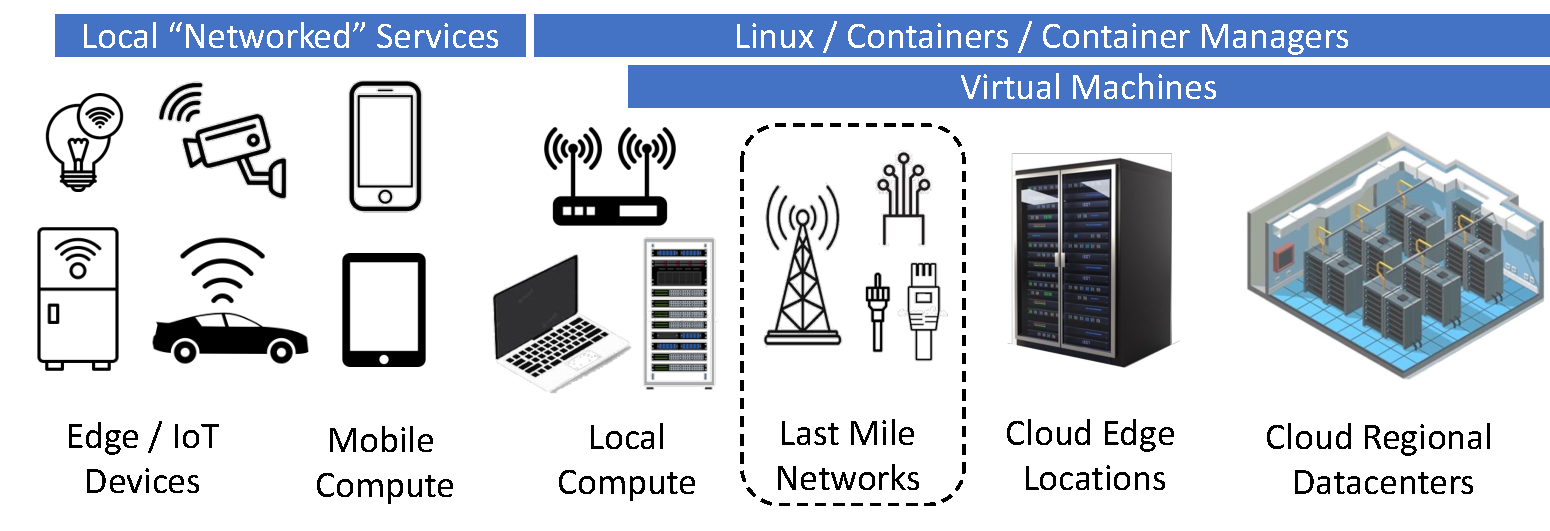
\includegraphics[width=\textwidth]{images/CloudTopo2.pdf}	
	\caption{Cloud Compute - From Big to Small}
	\label{fig:CloudTopo}
\end{figure*}

The infrastructure architecture that the major cloud providers offer to their customers continues to expand and evolve.  These advancements provide significant innovation capabilities to their customers, but also put pressure on how to effectively engineer solutions that take advantage of these services cost effectively.  Figure \ref{fig:CloudTopo} shows the high level view of the modern cloud.  While it was once easy to identify the boundary of where the cloud started and ended, it is no longer easy to define the edge of the cloud.  The following sections will provide an overview of the evolution of the cloud, along with highlighting some of the challenges that have to be overcome by software engineers to effectively use cloud computing services in their products.

\subsection{Foundational Cloud Architecture}

The basic cloud architecture topology deployed by the major providers exhibit a lot of similarities\footnote{It should be noted that the terminology used by the major cloud providers differs slightly for things like availability zones and regions.}.  The foundational building block of cloud compute is often called an \textbf{Availability Zone} (AZ).  An AZ is a data center that hosts cloud infrastructure (compute, storage, and network) and runs cloud provider services.  A \textbf{Region} is a physical location where a collection of 2 or more AZs are located.  Each AZ within a region are connected together with a fully redundant high bandwidth low latency network.  The goal of a region is to have AZs close enough so that they can behave like a single cluster, but also separate them by enough distance to isolate them from issues associated with power failure, earthquakes, tornados, and so on.  AWS, as an example, uses the general guideline of 100km (60 miles)\cite{AWS-AZ} for placing AZs within a region. The global footprint of a cloud provider is defined by the number of regions and locations they have across the globe, along with the purpose-built underlying network they use to interconnect them together. The far right side of Figure \ref{fig:CloudTopo} shows where Regions and AZs fit into the modern cloud architecture.

The Region/AZ architecture, coupled with a pay-as-you-go model, offered services, scale and financial benefits that disrupted compute.  The largest companies in the world do not want to be in the business of managing a global network of interconnected data centers. For smaller companies and individual entrepreneurs, this model enabled them to have access to compute resources once only available to large enterprises, for zero up front cost.  One could easily argue that cloud computing was largely responsible for the explosion in startup companies over the past 15-20 years. 

From a software engineering perspective, the basic cloud architecture introduces additional cognitive load on engineers:

\begin{itemize}
	\item Planning application deployment starts with the design of a virtual data center. Traditional software engineers are not trained to think of the start of the design process begins with the assignment of a network CIDR block. Historically, the physical network and security topology was designed by others and fixed, and was inherited "as is" into the final software architecture. 
	
	\item Quality attributes such as privacy, resiliency, reliability and scalability are foundational concepts that software architects use to reason about systems.  These now move out of the conceptual realm and require a deeper understanding of technical constructs that now become part of the software design itself.  For example, deploying microservices across different subnets, where each subnet is in a different AZ within a region. Also, declarative definition of  the security policies that govern access to these microservices along with their entitlements to access other cloud resources becomes part of the software product itself. 
	
	\item Although the cloud itself provides an infrastructure model to create resilient solutions that run at scale, its up to the software engineer to build things properly to take advantage of these capabilities\footnote{Some patterns such as rehosting\cite{engelsrud2019moving} {\em a.k.a.} "lift-and-shift" have emerged that contrast the benefits of moving workloads to the cloud with unplanned for consequences such as higher operational costs and little to no improvement in resiliency.}.  For example, it's still possible to deploy an application to a single virtual machine instance in the cloud, which will not elastically scale, nor will it be resilient to failure.  Thus, to enable the creation of cloud services software engineers must have mastery of newer patterns for distributed applications ( {\em e.g.}, asynchronous event-based architectures).
	
	\item One clear benefit of deploying to the cloud is that the easiest path to do so requires everything to be automated. 
	
\end{itemize}


Within a ge
Although terminology In the early days of the cloud the boundaries of where the cloud started and ended were clear. Cloud providers provided multiple clustered datacenters, often called Availability Zones (AZ), and  

The physical architecture of the cloud is materially different from what students are exposed to in a traditional computer science or software engineering program.  Figure \ref{fig:CloudTopo}.

\subsection{Expanding the edge of the cloud}
As cloud providers expand their footprint across the globe, creating new regions with multiple availability zones represents an expensive and time consuming investment. Creating new regions is required to increase compute capacity as global cloud adoption expands, and to meet specific compliance requirements associated with conducting business in the cloud. For example, many countries are adopting data residency laws, which place controls over where data is stored at rest. 

In many cases, new regions are not required, but cloud applications continue to push for better performance, which in many cases needs to be achieved via providing lower latency.  Approaches to lower latency have been deployed before the modern cloud with content delivery network (CDN)\cite{CDN} solutions. 

\section{Cloud Native Requires Embracing "Polyglot"}
Underlying HW runtime diversity, Microcontrollers, etc
\subsection{Polyglot Programming}
blah

\subsection{Polyglot Databases}
blah

\subsection{Polyglot Hardware}
blah
Docker - AMD and ARM
AWS - Graviton
Edge Computing - Microcontrollers - Go/Rust


\section{Software Architecture Requirements}
\label{sec:SoftwareArchitecture}

\section{Software Construction Requirements}
\label{sec:SoftwareConstruction}

\subsection{Polyglot Programming}
\label{subsec:Polyglot}

\section{Temporary Stuff}
It's been less than 20 years since the reality of "compute as a utility" provided by the cloud, and the universal acceptance of integrating open source software into commercial applications. With the cloud, and modern 

For example, better software can loosely be defined as software that meets its documented requirements with as few defects as possible.  Prior to the ability to distribute and patch software over the internet, significant defects required expensive measures to address.  Software providers would need to create updates and ship them to all of their customers using physical media such as disks, tapes or CD/DVD media.  We see these complex and costly defect management techniques in other industries such as managing automotive recalls. Given these challenges, extensive governance over feature scope and aggressive correctness testing were needed to avoid these emergency patches.  Delivering faster is often treated as compromising quality in order to maximize features. Optimizing around cost generally drove tradeoffs in areas such as being able to run on existing infrastructure, minimizing scope, or minimizing testing as the effort to patch defects became simpler. 

While the innovations associated with the cloud and open source software have undoubtedly advanced the software profession, traditional software engineering practices have been slow to evolve.  We think there is significant opportunity to evolve the state of the art in software engineering given the likelihood that most industrial systems moving forward will be deployed on cloud runtimes\footnote{By cloud runtime we include public, private and hybrid cloud infrastructure}. Specifically:

\begin{itemize}
	\item Helping Software Engineers manage the expanded cognitive required to design, build and deploy at scale cloud applications.
	\item Identify opportunities to accelerate and scale software engineering skillsets needed for the cloud. Many industries will strive to move beyond deploying e-commerce applications to the cloud with their top engineers. This will require developing new skills for the broader engineering organization.
	\item Investigate how software engineering and computer science education can expand to address the needs of industry in creating cloud-ready software engineering professionals. 
\end{itemize}



\bibliography{CloudNative.bib}
\end{document} 